\documentclass[../taasin.tex]{subfiles}
\graphicspath{{\subfix{../figures/}}}
\begin{document}

We test if our SNN foveation controller can produce 3 of the eye movements used in \cite{Arjun}'s thesis. We run our SNNs with both the normal ONV and the delta ONV, using LiNet performance as a baseline to compare to.

%%%%%%%%%%%%%%%%%%%%%%%%%%%%%%%%%%%%%%%%%%%%%%%%%%%%%%%%%%%%%%%%%%%%%%

\subsection{Fixation}

This test does not involve any movement of the target. We keep the target still and observe how well it is kept in the center of the retina. An unrealistic model would fixate perfectly on the ball and not move, whereas a more realistic model would allow the target to drift around the center of the fovea. These small movements are similar to micro-saccades in real eyes where a movement in one direction is balanced with a consecutive movement in the opposite direction. Figure \ref{fig:fixation}  shows this type of movement across four timesteps.

% TODO: describe figure more

\begin{figure}
    \centering
    \begin{subfigure}[b]{0.20\textwidth}
        \centering
        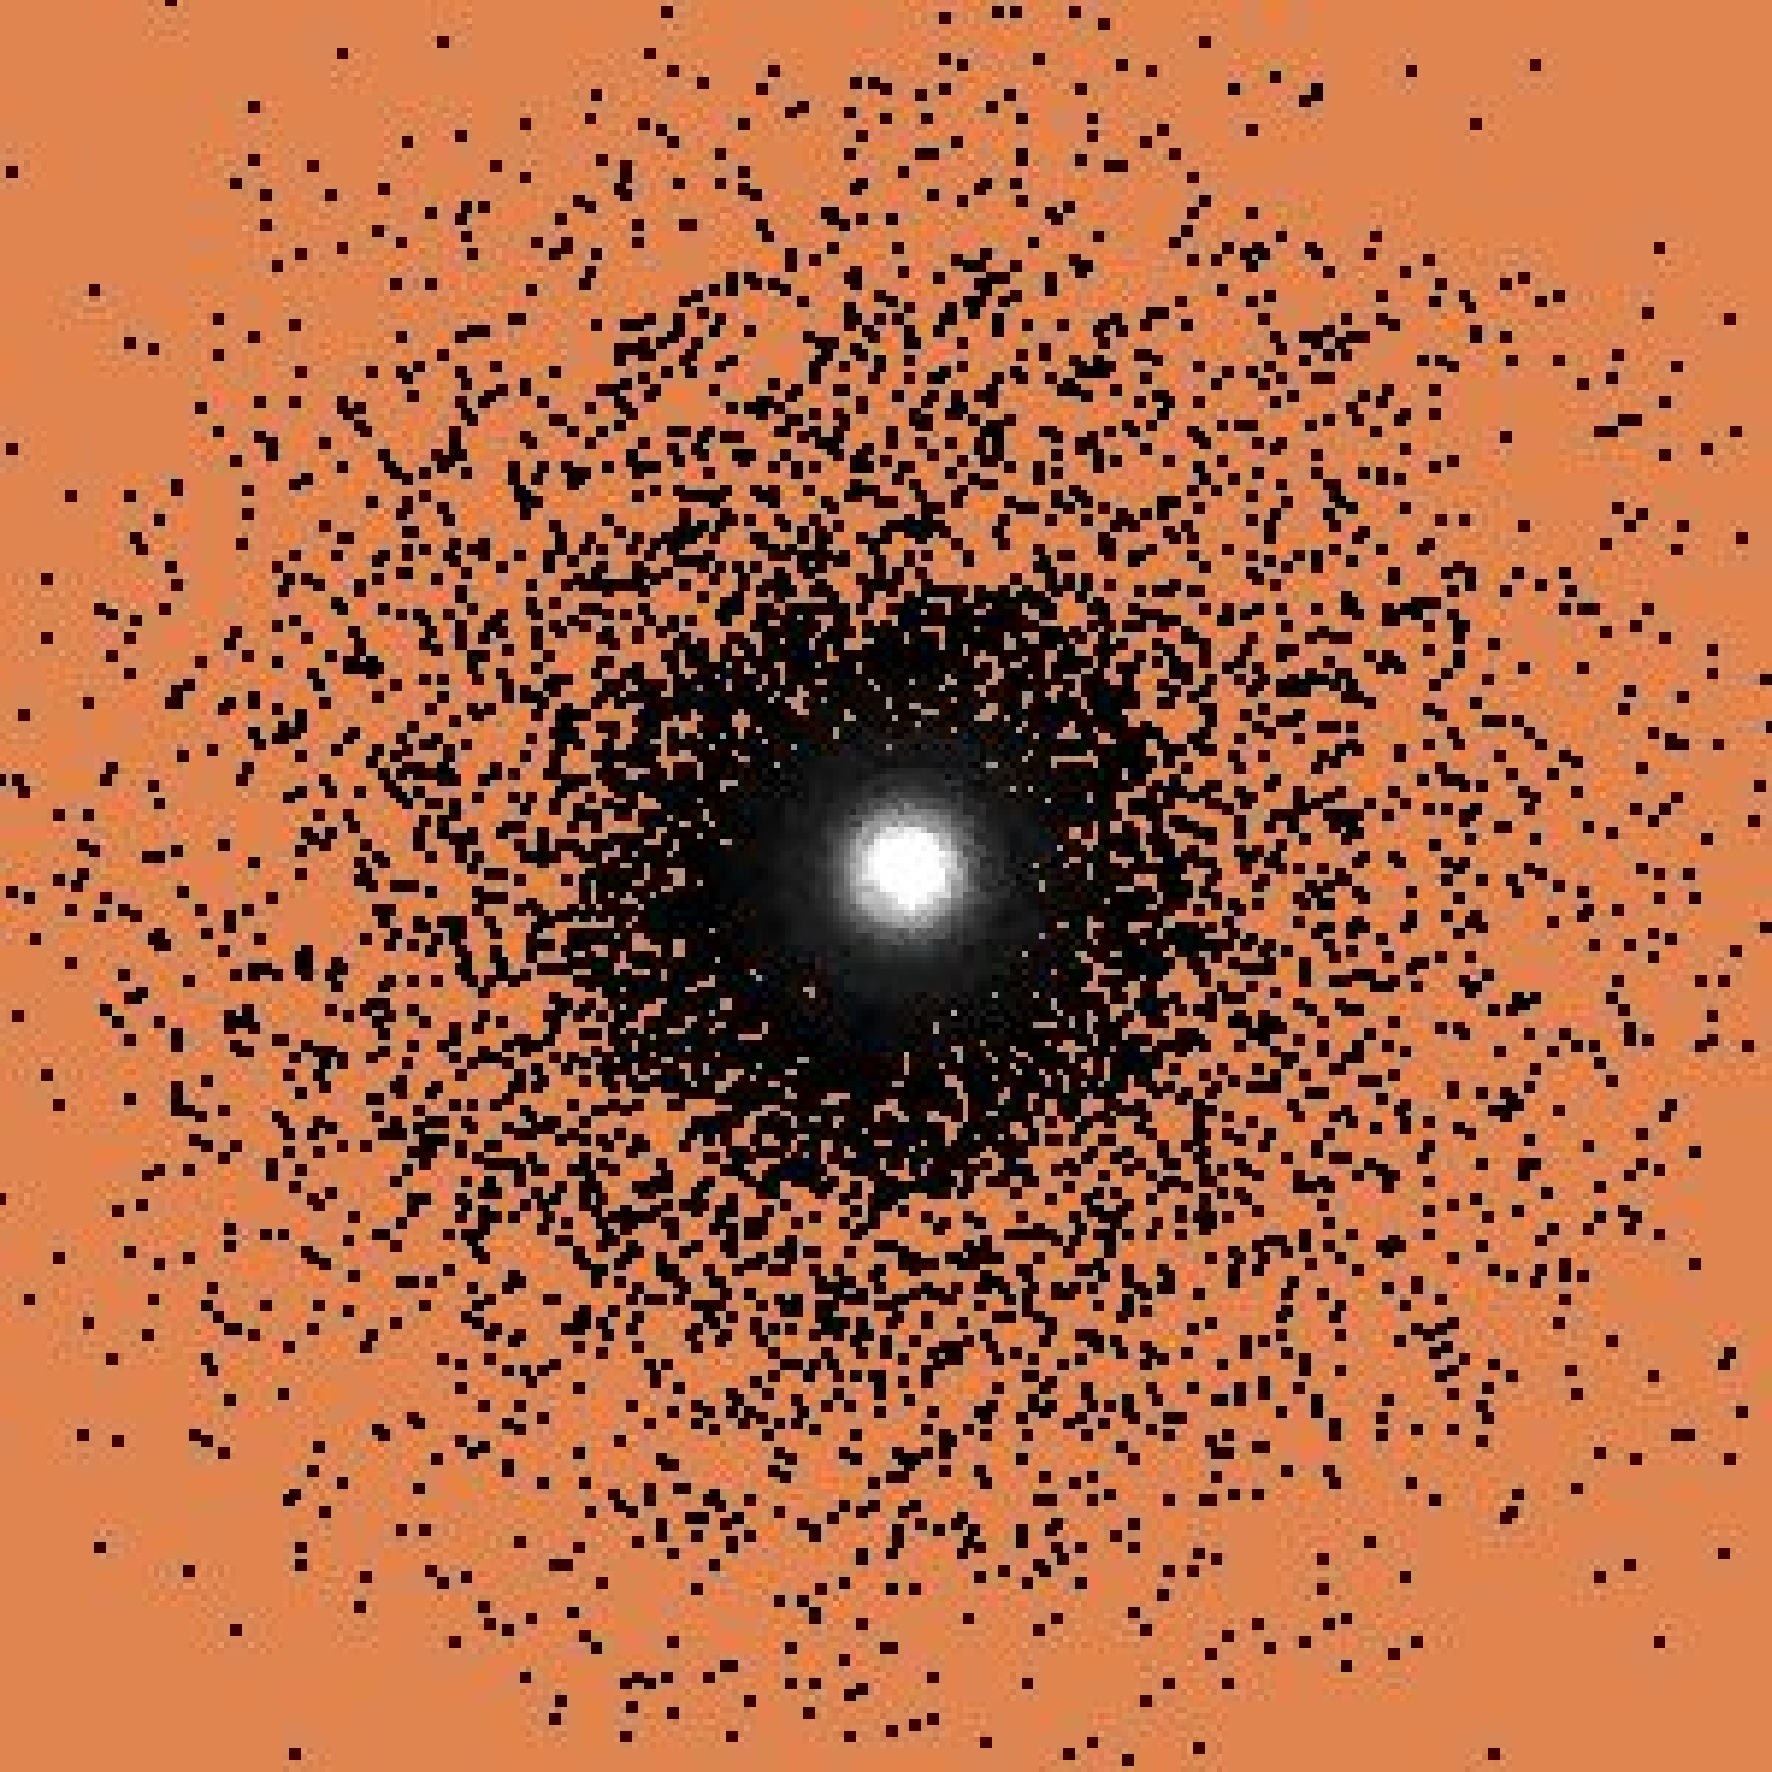
\includegraphics[width=\textwidth]{figures/fixation1.pdf}
        \caption{}
    \end{subfigure}
    \hfill
    \centering
    \begin{subfigure}[b]{0.20\textwidth}
        \centering
        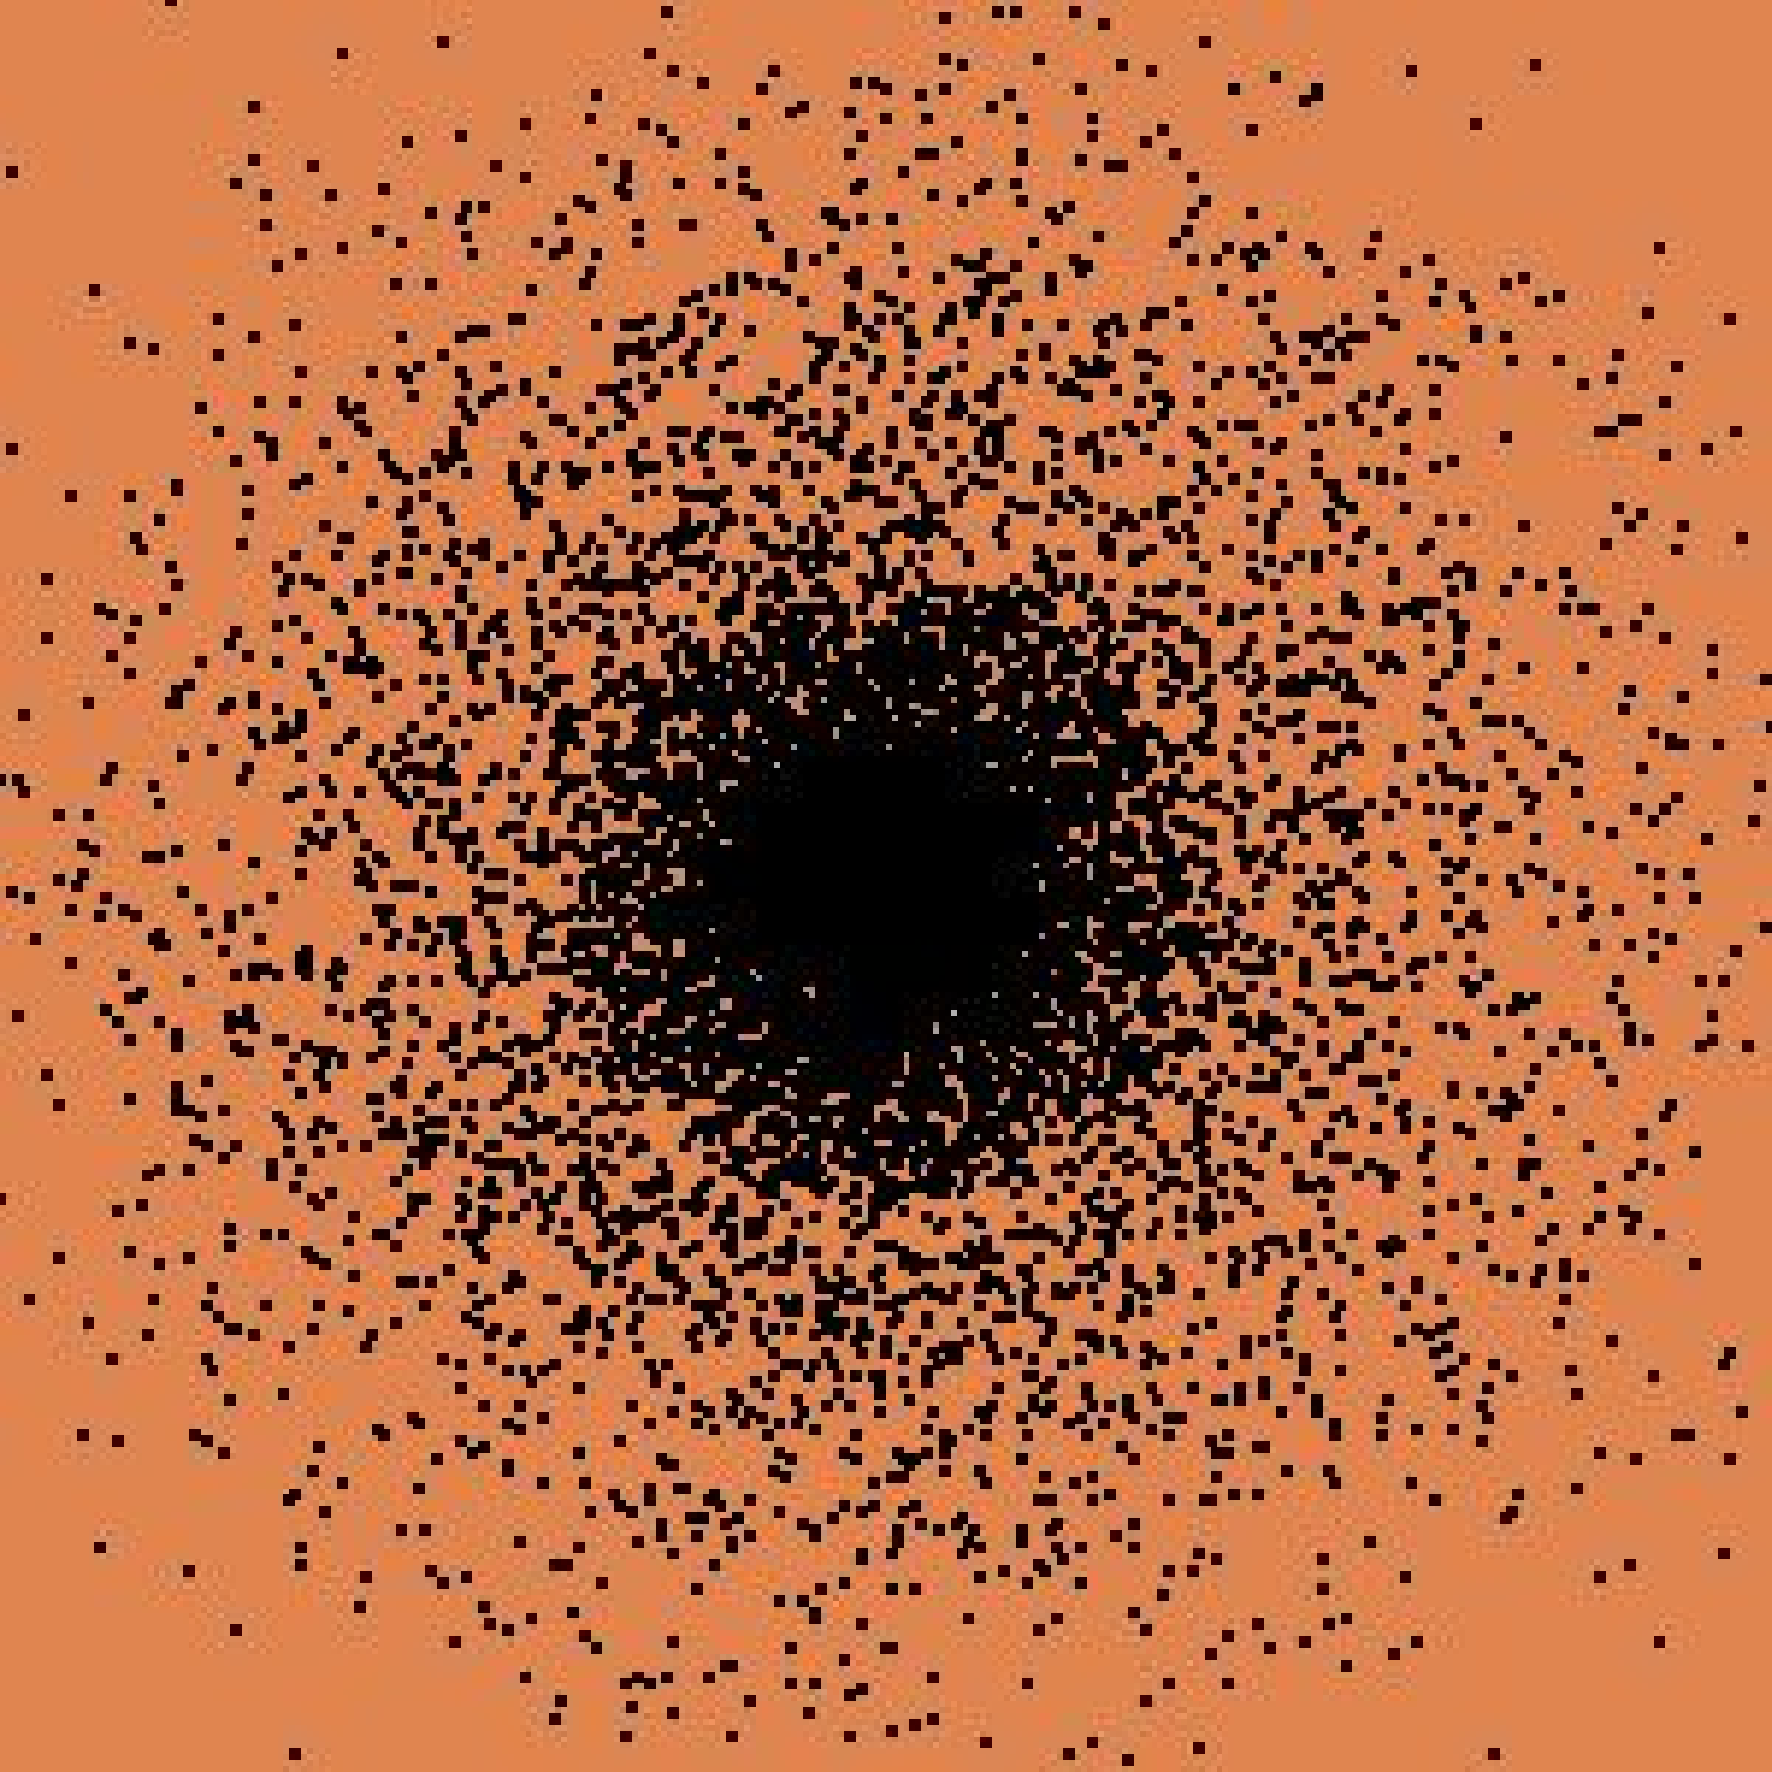
\includegraphics[width=\textwidth]{figures/fixation2.pdf}
        \caption{}
    \end{subfigure}
    \hfill
    \centering
    \begin{subfigure}[b]{0.20\textwidth}
        \centering
        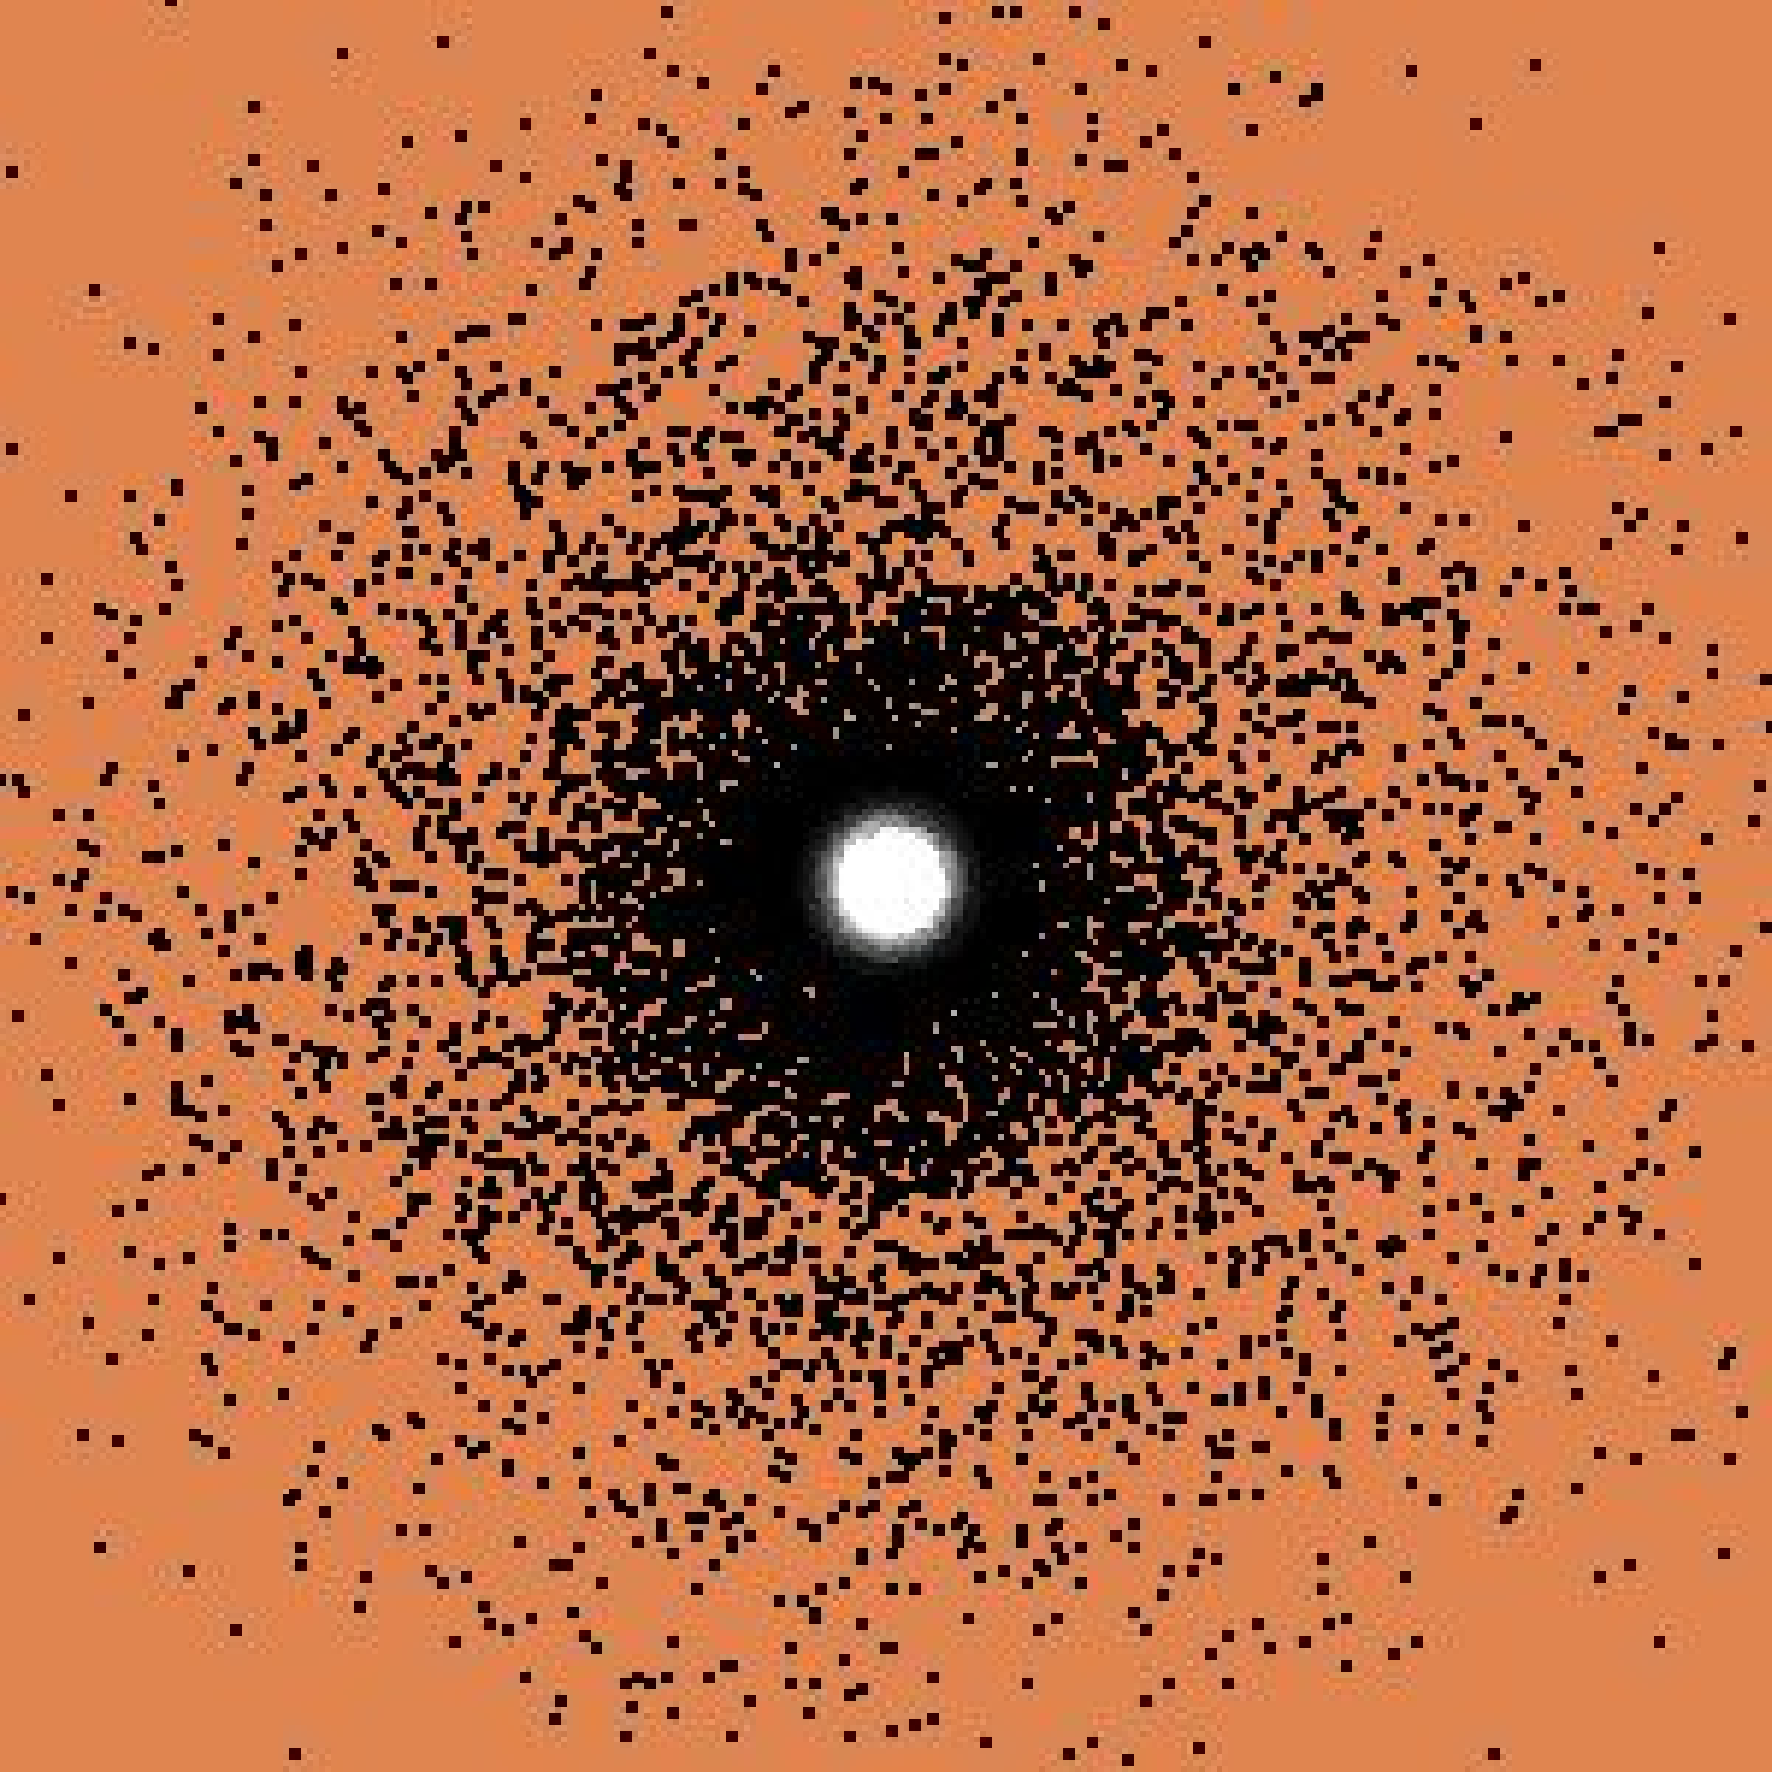
\includegraphics[width=\textwidth]{figures/fixation3.pdf}
        \caption{}
    \end{subfigure}
    \hfill
    \centering
    \begin{subfigure}[b]{0.20\textwidth}
        \centering
        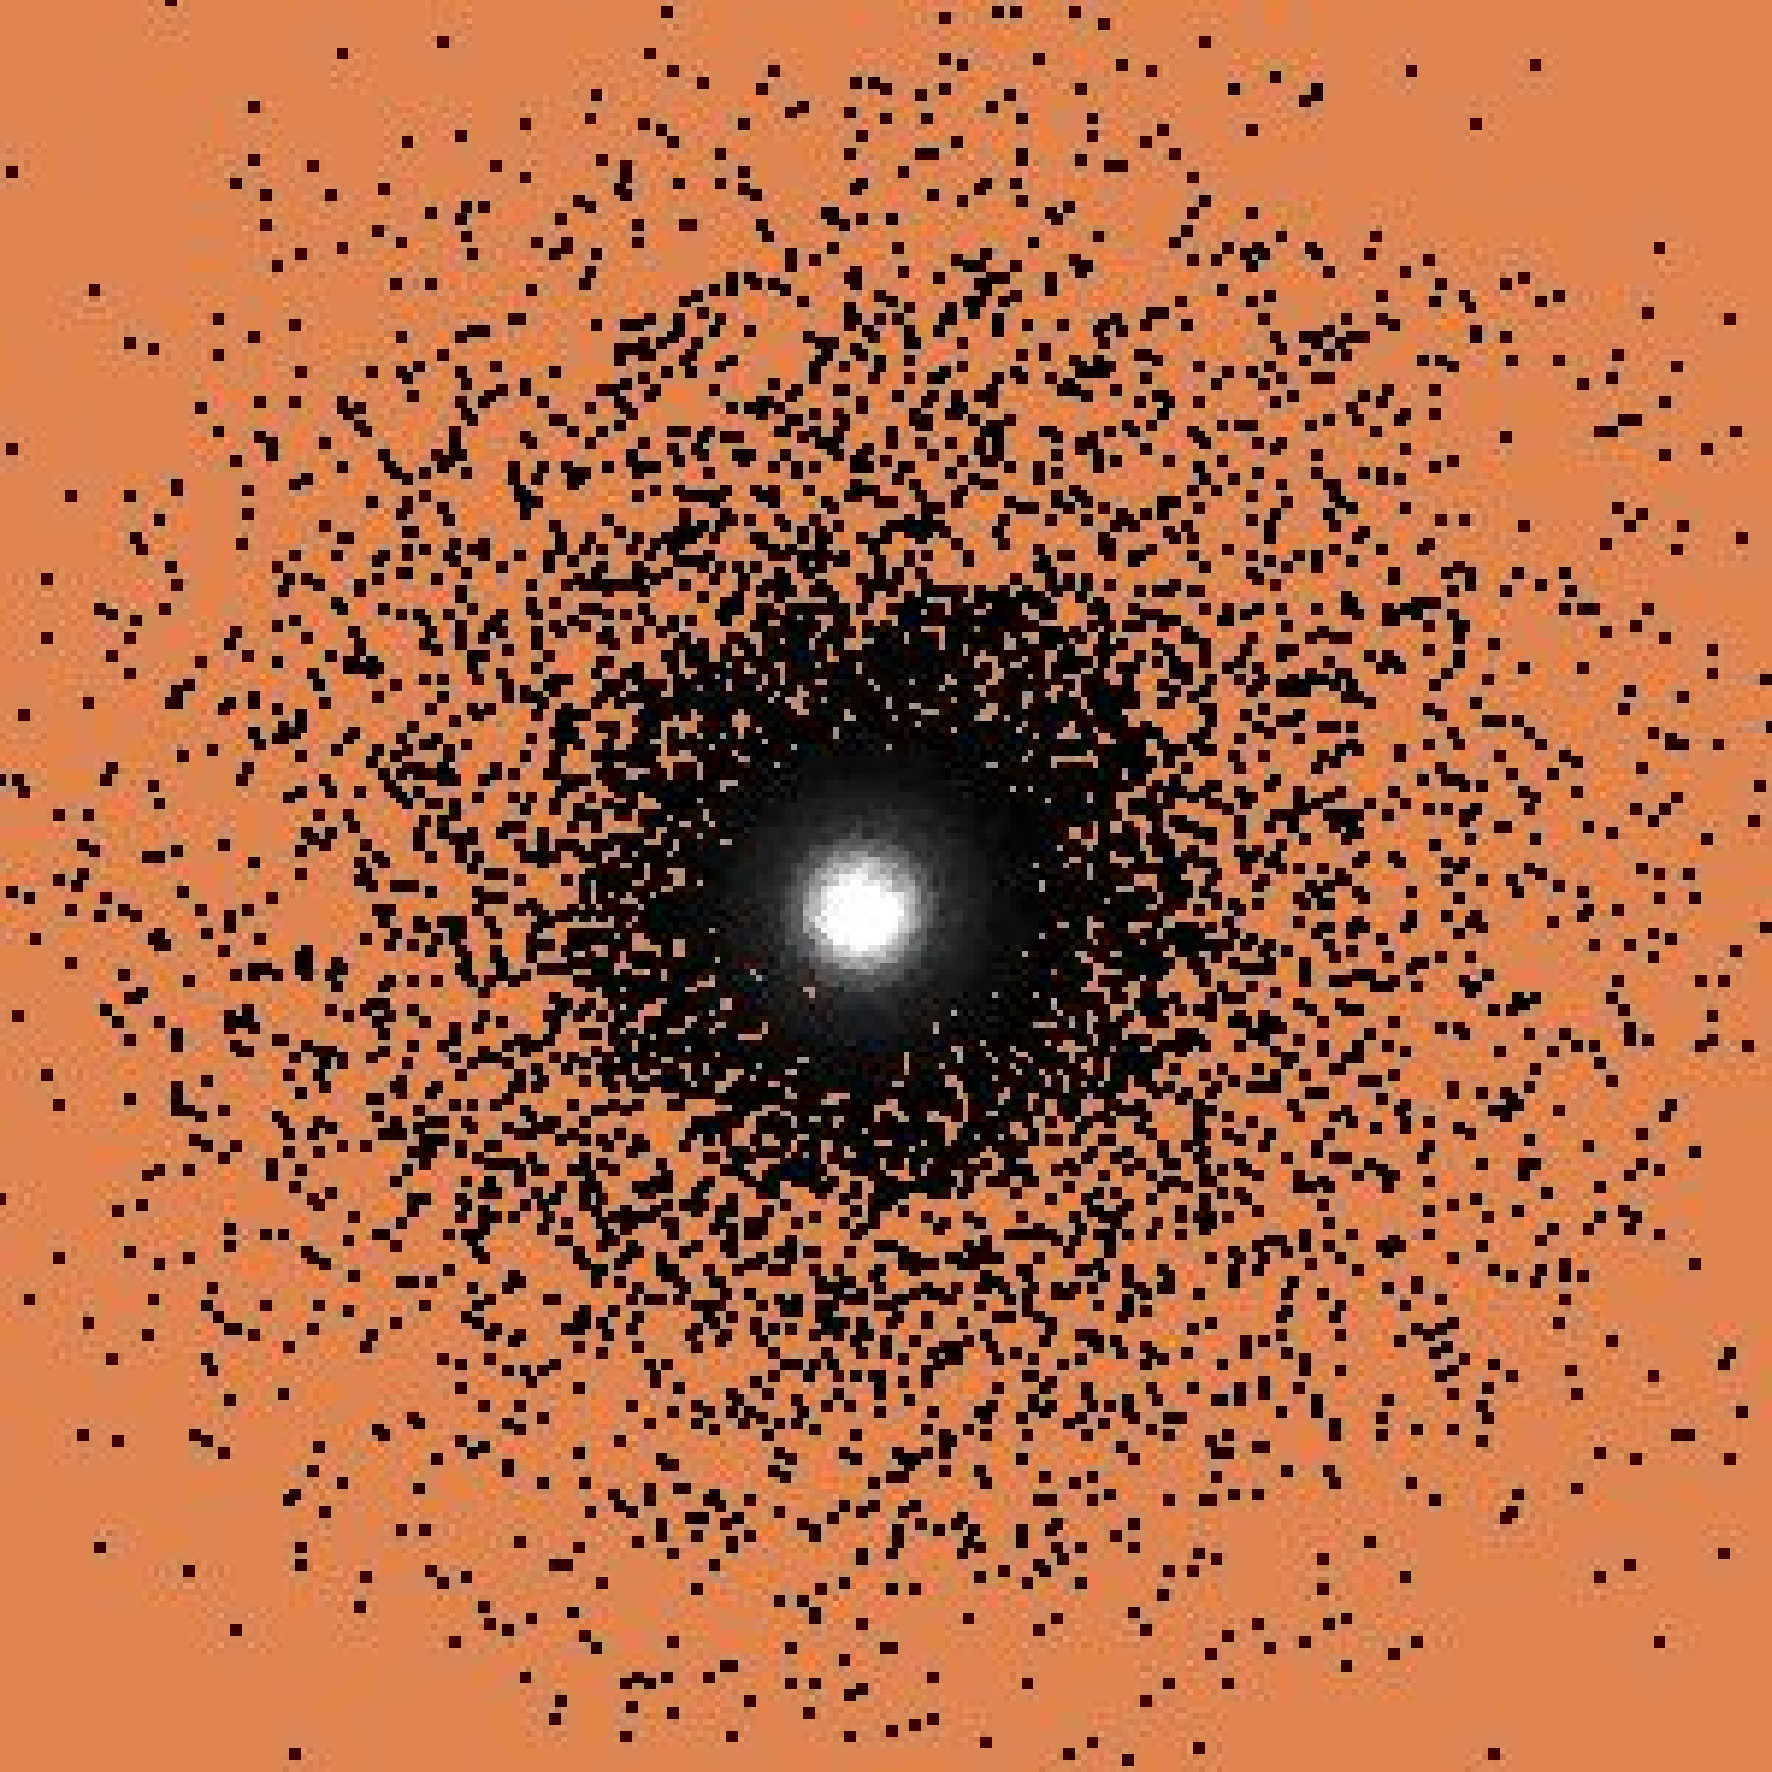
\includegraphics[width=\textwidth]{figures/fixation4.pdf}
        \caption{}
    \end{subfigure}
    \caption{In (a), the ball has just entered the eye's field of view. In (b) the eye has fixated on the ball. In (c)-(d) we see micro-saccades in opposite directions.}
    \label{fig:fixation}
\end{figure}

%%%%%%%%%%%%%%%%%%%%%%%%%%%%%%%%%%%%%%%%%%%%%%%%%%%%%%%%%%%%%%%%%%%%%%

\subsection{Smooth Pursuit}

The smooth pursuit test moves the target slowly in both the horizontal and vertical directions. We observe if our SNN can successfully track this motion with $\theta$ and $\phi$ changing at the same time.

In figure \ref{fig:smooth} we compare the performance of a LiNet to that of our 4 layer SNN. The black lines represent the exact position that the eye's gaze should move at each timestep. The orange lines track the performance of the LiNet architecture and the blue lines track the performance of our SNN. 

In figure \ref{fig:smooth_normal} we compare the performance on the normal ONV. The LiNet performs much better here. In figure \ref{fig:smooth_delta} the SNN performs better with a delta ONV but we note that the motions are more noisy. Finally, in figure \ref{fig:smooth_hybrid} we see that adding just one layer with a ReLU activation results in smooth performance using the delta ONV.

\begin{figure}
    \centering

    \begin{subfigure}[b]{0.5\textwidth}
        \centering
        \includegraphics[width=\textwidth]{figures/smooth_ori_normal.pdf}
        \caption{}
        \label{fig:smooth_normal}
    \end{subfigure}

    \hfill

    \begin{subfigure}[b]{0.5\textwidth}
        \centering
        \includegraphics[width=\textwidth]{figures/smooth_ori_delta.pdf}
        \caption{}
        \label{fig:smooth_delta}
    \end{subfigure}

    \hfill

    \begin{subfigure}[b]{0.5\textwidth}
        \centering
        \includegraphics[width=\textwidth]{figures/smooth_ori_delta_hybrid.pdf}
        \caption{}
        \label{fig:smooth_hybrid}
    \end{subfigure}

    \caption{We compare the output angles of the foveation controller in (a) and the orientation of the center of the eye in (b). The black line represents the expected output based on inverse dynamic simulation.}
    \label{fig:smooth}
\end{figure}

Our SNN, while noisy, tracks the target successfully. It also keeps the target in the center of the fovea when using the delta ONV.

%%%%%%%%%%%%%%%%%%%%%%%%%%%%%%%%%%%%%%%%%%%%%%%%%%%%%%%%%%%%%%%%%%%%%%

\subsection{Saccade}

In a real saccade, the eye move rapidly in different directions. To re-create this movement, we allow the eye to fixate on the ball and then rapidly move it to a new point within the eye's field of view. 

In figure \ref{fig:saccade} we again compare the performance of a LiNet to that of our 4 layer SNN.
In figure \ref{fig:saccade_normal} we compare the performance on the normal ONV. The LiNet performs much better here. In figure \ref{fig:saccade_delta} the SNN performs better with a delta ONV but we note that the motions are more noisy. Finally, in figure \ref{fig:saccade_hybrid} we see that adding just one layer with a ReLU activation results in smooth performance using the delta ONV.

\begin{figure}
    \centering

    \begin{subfigure}[b]{0.5\textwidth}
        \centering
        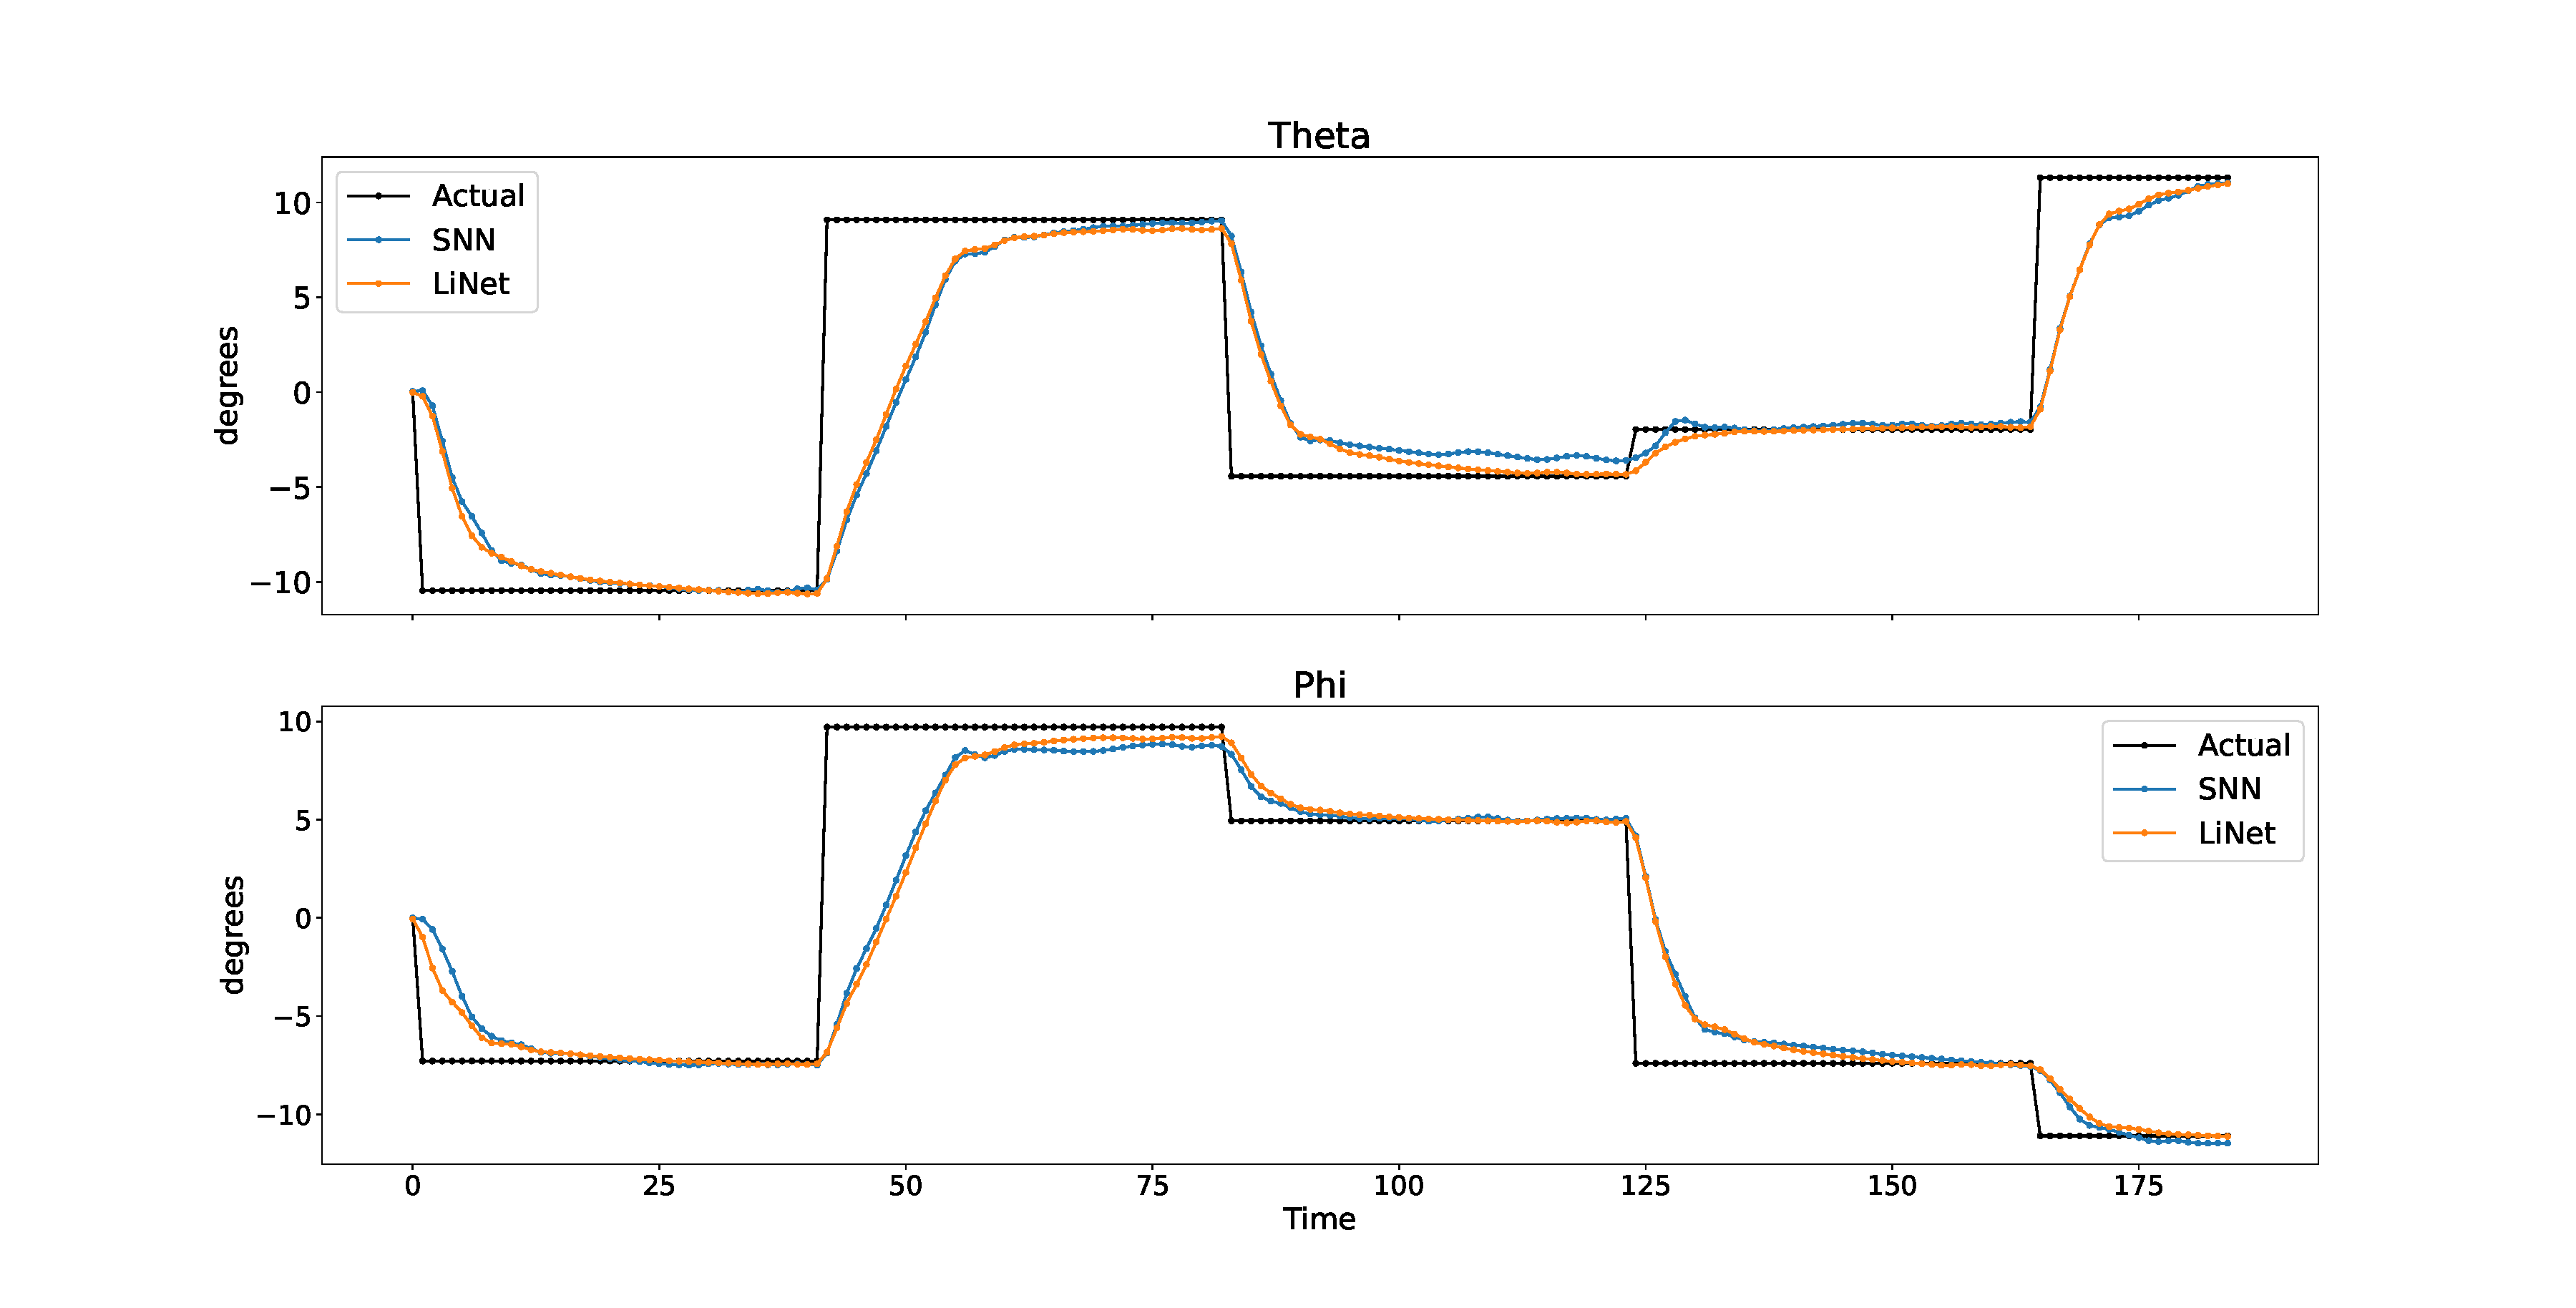
\includegraphics[width=\textwidth]{figures/saccade_normal.pdf}
        \caption{}
        \label{fig:saccade_normal}
    \end{subfigure}

    \hfill

    \begin{subfigure}[b]{0.5\textwidth}
        \centering
        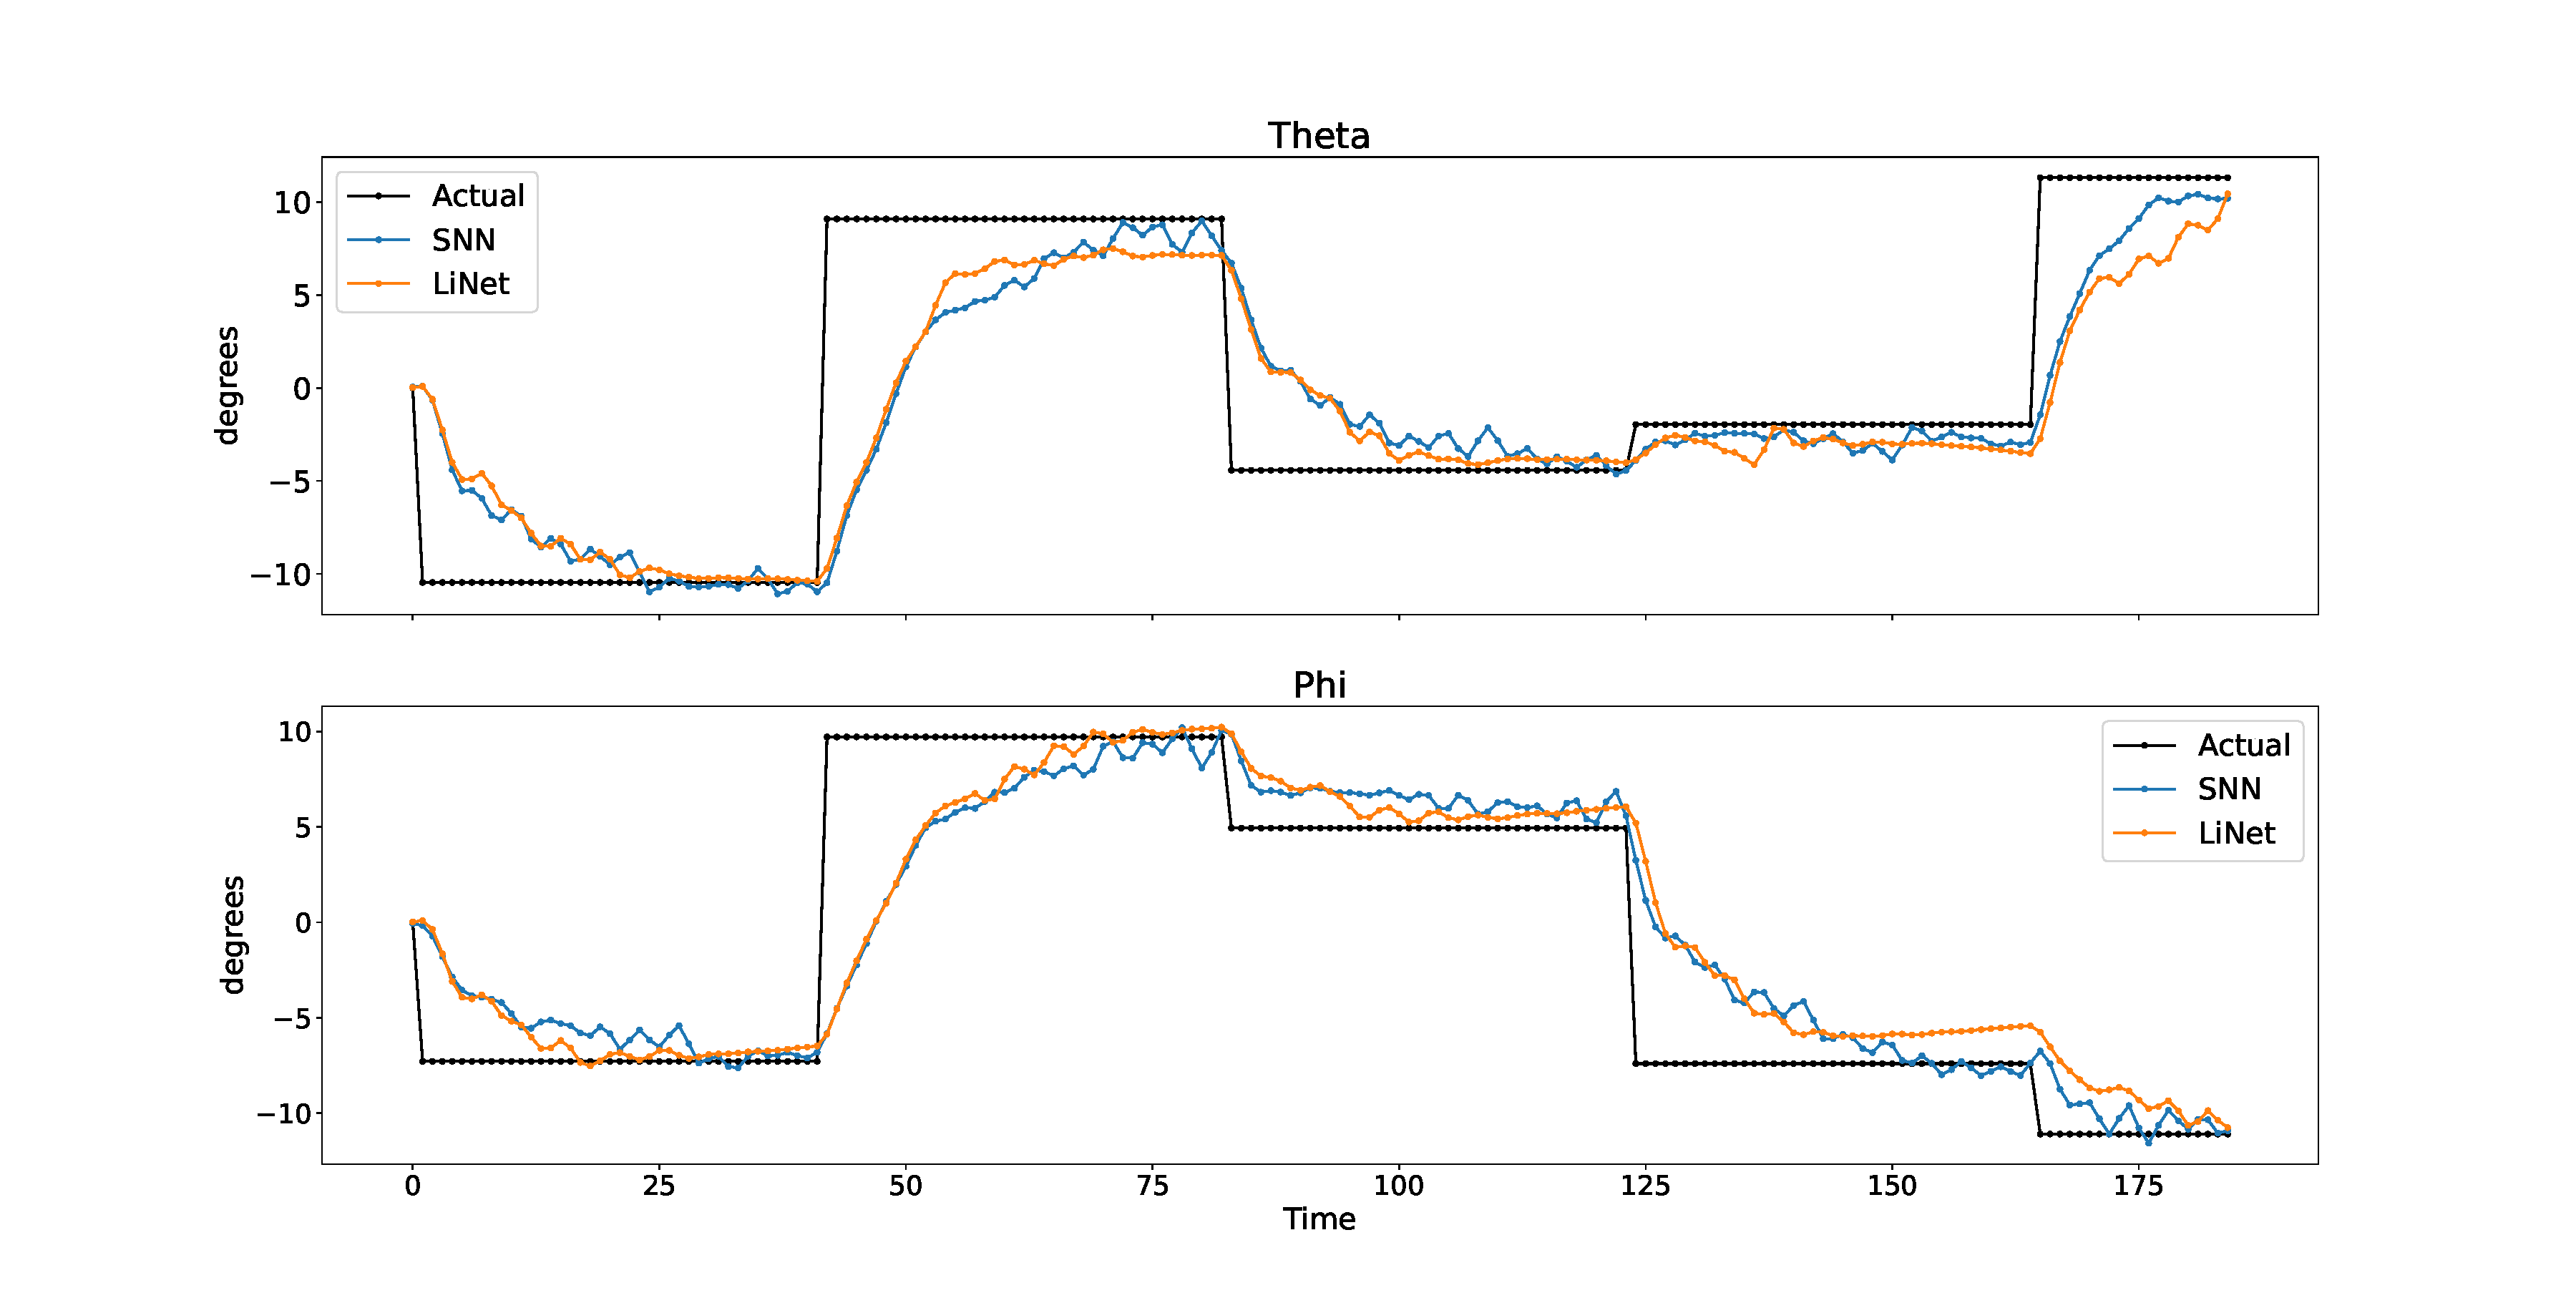
\includegraphics[width=\textwidth]{figures/saccade_delta.pdf}
        \caption{}
        \label{fig:saccade_delta}
    \end{subfigure}

    \hfill

    \begin{subfigure}[b]{0.5\textwidth}
        \centering
        \includegraphics[width=\textwidth]{figures/saccade_hybrid.pdf}
        \caption{}
        \label{fig:saccade_hybrid}
    \end{subfigure}

    \caption{We compare the output angles of the foveation controller in (a) and the orientation of the center of the eye in (b). The black line represents the expected output based on inverse dynamic simulation.}
    \label{fig:saccade}
\end{figure}

Our SNN, while noisy, tracks the target successfully. It also keeps the target in the center of the fovea when using the delta ONV.

We also use the saccade test to evaluate how realistic our eye movements are.

%%%%%%%%%%%%%%%%%%%%%%%%%%%%%%%%%%%%%%%%%%%%%%%%%%%%%%%%%%%%%%%%%%%%%%

\subsection{Projectile Motion}

%%%%%%%%%%%%%%%%%%%%%%%%%%%%%%%%%%%%%%%%%%%%%%%%%%%%%%%%%%%%%%%%%%%%%%

\subsection{SNN Analysis}

% look at thresholds, membranes, spike rates?

%%%%%%%%%%%%%%%%%%%%%%%%%%%%%%%%%%%%%%%%%%%%%%%%%%%%%%%%%%%%%%%%%%%%%%

% compare membrane voltage graphs to actual retinal spikes?

\end{document}